% ft-12-Optimization.tex

\documentclass[xcolor=dvipsnames]{beamer}
\usepackage{teachbeamer}

\title{Optimization and Analyzing Functions}
\subtitle{{\CourseNumber}, BCIT}

\author{\CourseName}

\date{November 13, 2018}

\begin{document}

\begin{frame}
  \titlepage
\end{frame}

\begin{frame}
  \frametitle{Relative Extrema}
A function $f$ has a \alert{relative maximum} at $x=c$ if there exists
an open interval $(a,b)$ containing $c$ such that $f(x)\leq{}f(c)$ for
all $x$ in $(a,b)$.

\bigskip

A function $f$ has a \alert{relative minimum} at $x=c$ if there exists
an open interval $(a,b)$ containing $c$ such that $f(x)\geq{}f(c)$ for
all $x$ in $(a,b)$.
\end{frame}

\begin{frame}
  \frametitle{Derivatives and Extrema}
  At any number $c$ where a differentiable function $f$ has a relative
  extremum, $f'(c)=0$. The converse is not true. Consider the
  following two functions and their derivatives.
\begin{equation}
  \label{eq:thapoich}
f_{1}(x)=x^{3}+x^{2}-5x-1
\end{equation}
\begin{equation}
  \label{eq:gohshaem}
f_{2}(x)=\left(\frac{3}{10}x\right)^{3}
\end{equation}
\end{frame}

\begin{frame}
  \frametitle{Derivatives and Extrema Graph I}
  \begin{figure}[h]
    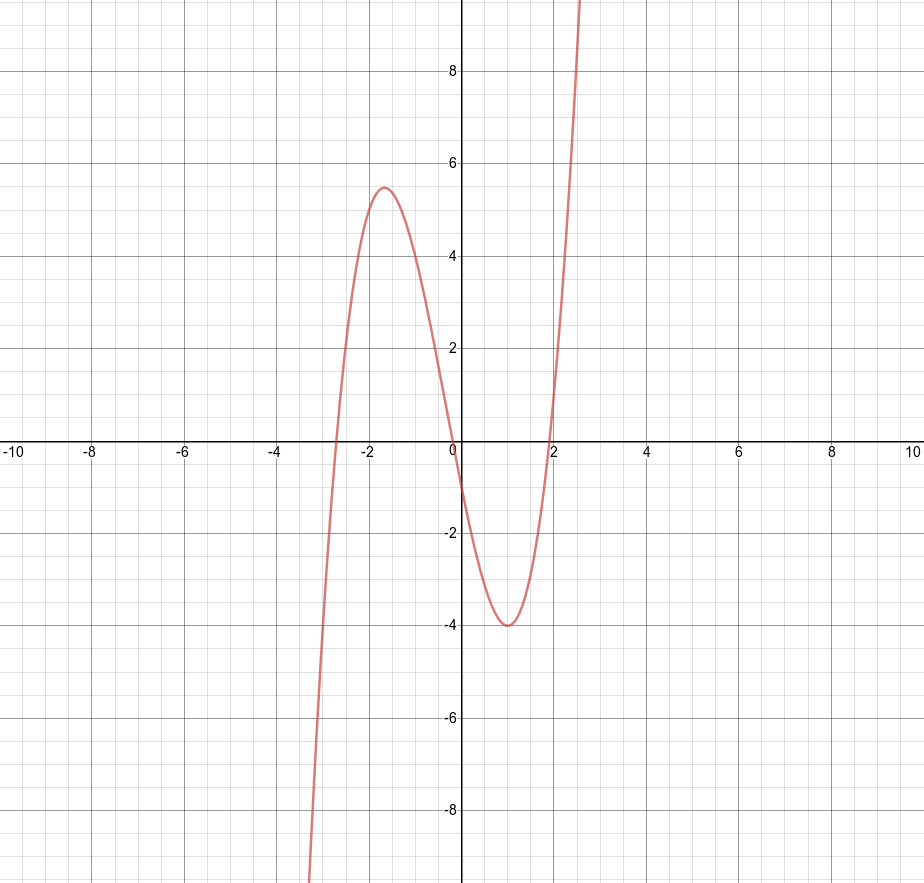
\includegraphics[scale=.3]{./extrema1.png}
  \end{figure}
\end{frame}

\begin{frame}
  \frametitle{Derivatives and Extrema Graph II}
  \begin{figure}[h]
    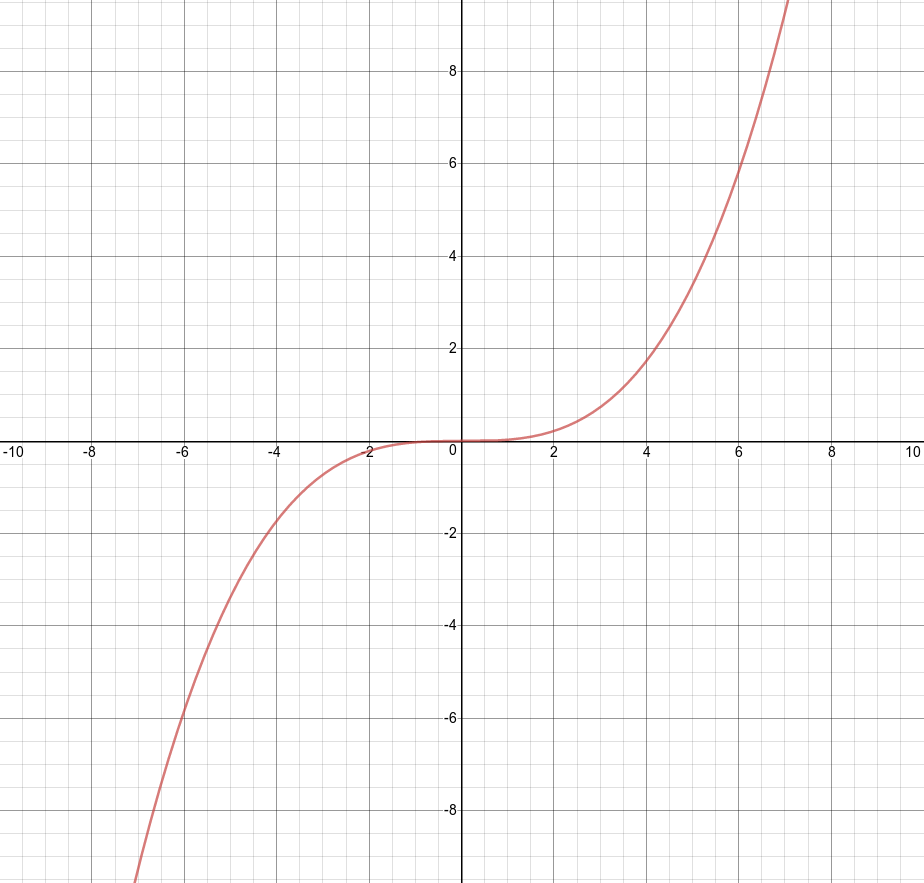
\includegraphics[scale=.3]{./extrema2.png}
  \end{figure}
\end{frame}

\begin{frame}
  \frametitle{Derivatives and Extrema Caution}
Note that a function may have an extremum at a point where the
derivative is not $0$ if at that point the function is not
differentiable. Consider this function and its derivative.
\begin{equation}
  \label{eq:ceezukoh}
f_{3}(x)=x^{\frac{2}{3}}
\end{equation}
\begin{block}{Critical Number}
  A \alert{critical number} of a function $f$ is any number $x$ in the
  domain of $f$ such that $f'(x)=0$ or $f'(x)$ does not exist.
\end{block}
\end{frame}

\begin{frame}
  \frametitle{Derivatives and Extrema Graph III}
  \begin{figure}[h]
    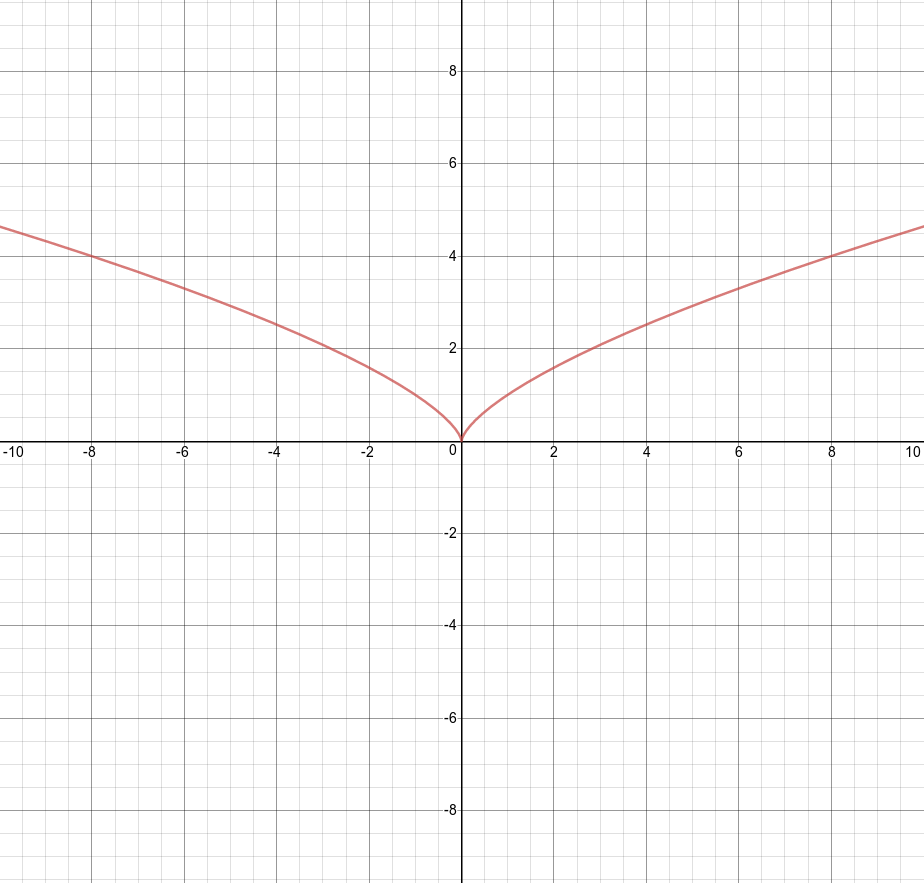
\includegraphics[scale=.3]{./extrema3.png}
  \end{figure}
\end{frame}

\begin{frame}
  \frametitle{Extrema Exercises}
Find the relative maxima and relative minima, if any, of each
function.
\begin{equation}
  \label{eq:xoongohh}
f(x)=x^{3}-4x
\end{equation}
\begin{equation}
  \label{eq:aghuomoh}
h(t)=-t^{2}+6t+6
\end{equation}
\begin{equation}
  \label{eq:yakovuap}
f(x)=\frac{1}{2}x^{4}-x^{2}
\end{equation}
\begin{equation}
  \label{eq:aweefahx}
g(x)=\frac{x+1}{x}
\end{equation}
\begin{equation}
  \label{eq:ebukatio}
f(x)=x\sqrt{x-4}
\end{equation}
\begin{equation}
  \label{eq:inaidimo}
h(s)=s^{\frac{5}{3}}
\end{equation}
\end{frame}

\begin{frame}
  \frametitle{Analyzing Functions}
To analyze a function, determine the following features:
\begin{itemize}
\item Domain and range of the function.
\item Zeros (also called $x$-intercepts) of the function.
\item Critical points, maxima, minima.
\item Inflection points.
\item Asymptotes.
\item Is the function even ($f_{1}(x)=x^{2}+1$) or odd ($f_{2}(x)=x^{3}-x$)?
\end{itemize}
\end{frame}

\begin{frame}
  \frametitle{Analyzing Functions Step-By-Step I}
Here is a step-by-step guide to analyzing functions.
\begin{enumerate}
\item Determine the $x$-intercepts (also called zeros). Set $f(x)=0$
  and find the solution set.
\item Determine the critical points. Find the derivative $f'(x)$ and
  check whether there are points in the domain of $f$ that are not in
  the domain of $f'$. Then set $f'(x)=0$ and find the solution set.
\item Determine whether the critical points are maxima or minima or
  neither. Find $f''(x)$ and check whether $f''$ at the critical
  points is positive, negative, or neither. 
\end{enumerate}
\end{frame}

\begin{frame}
  \frametitle{Analyzing Functions Step-By-Step II}
Here is a step-by-step guide to analyzing functions.
\begin{enumerate}
\setcounter{enumi}{3}
\item Determine the inflection points. Set $f''(x)=0$ and find the
  solution set.
\item Determine the asymptotes. See next slide.
\item Determine whether, for all $x$ in the domain of $f$,
  $f(x)-f(-x)=0$ (in which case $f$ is even) or $f(x)+f(-x)=0$ (in
  which case $f$ is odd).
\item Using the information you have, and possibly a table of function
  values, graph the function. Then determine the domain and range of
  $f$.
\end{enumerate}
\end{frame}

\begin{frame}
  \frametitle{Finding Asymptotes I}
An asymptote is a linear function ($y=kx+d$ with slope $k$ and
$y$-intercept $d$) which the function graph of $f$ approaches. There
are three kinds of asymptotes.
\begin{block}{Vertical Asymptote}
  A vertical asymptote, strictly speaking, is not a linear function.
  It is a curve defined by $x=c$, where $c$ is a real number (we call
  real numbers like $c$ \alert{constants}). You can often find
  vertical asymptotes at points where $f$ is undefined.
\end{block}
Find vertical asymptotes by checking points which are not in the
domain of the function $f$. 
\begin{equation}
  \label{eq:peimoojo}
f(x)=\frac{1}{x-2}+3\mbox{ has an asymptote at }x=2
\end{equation}
\end{frame}

\begin{frame}
  \frametitle{Finding Asymptotes I}
Example:
\begin{equation}
  \label{eq:ohchamig}
f(x)=\frac{1}{x-2}+3\mbox{ has an asymptote at }x=2
\end{equation}
\begin{figure}[h]
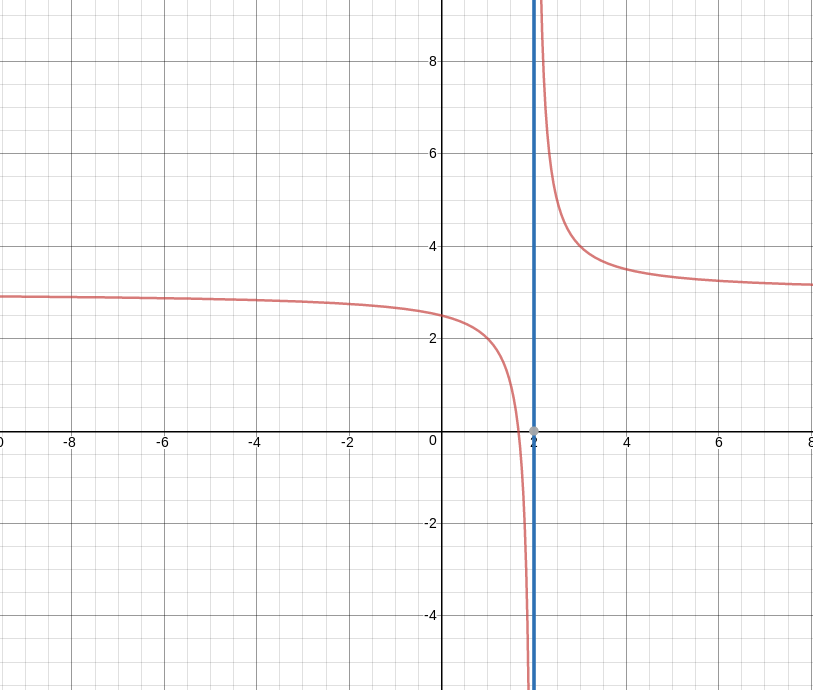
\includegraphics[scale=.25]{./asymp1.png}
\end{figure}
\end{frame}

\begin{frame}
  \frametitle{Finding Asymptotes I}
Example:
\begin{equation}
  \label{eq:aichohse}
f(x)=\ln(x+\pi)\mbox{ has an asymptote at }x=-\pi
\end{equation}
\begin{figure}[h]
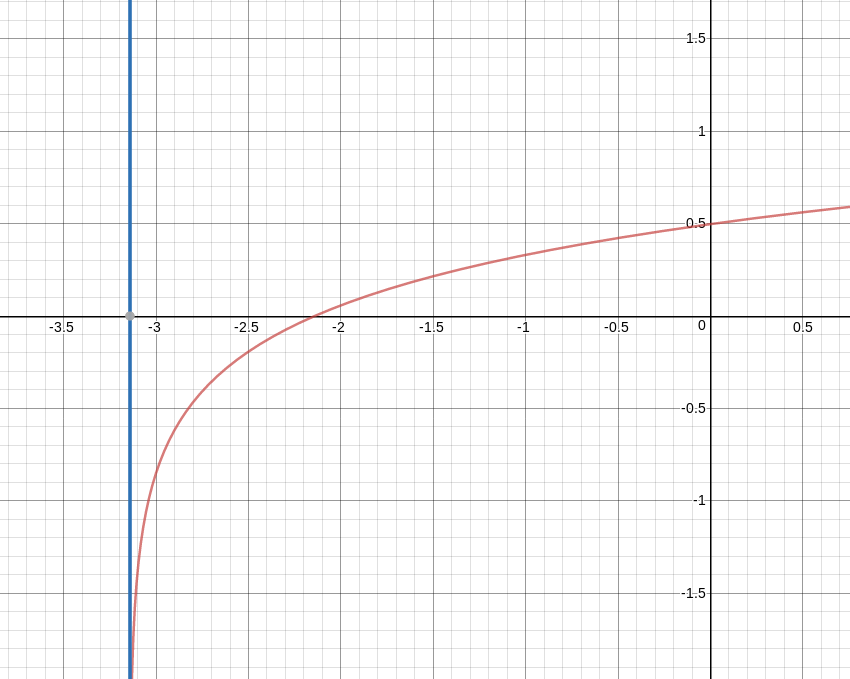
\includegraphics[scale=.25]{./asymp2.png}
\end{figure}
\end{frame}

\begin{frame}
  \frametitle{Finding Asymptotes II}
\begin{block}{Horizontal Asymptote}
  A horizontal asymptote is a linear function with slope $k=0$. Its
  equation is $y=c$, where $c$ is a constant. There are horizontal
  asymptotes for functions whose limits is a constant and for rational
  functions whose numerator and denominator polynomials share the same
  degree.
\end{block}
Find horizontal asymptotes by checking
\begin{equation}
  \label{eq:udaiguph}
  \lim_{x\rightarrow\infty}f'(x)\mbox{ and }\lim_{x\rightarrow{}-\infty}f'(x)
\end{equation}
If the limit is $k=0$, then that is also the slope of the asymptote.
\end{frame}

\begin{frame}
  \frametitle{Finding Asymptotes II}
Example
\begin{equation}
  \label{eq:tohwoiph}
f(x)=e^{\frac{x}{2}}+7\mbox{ has the asymptote }y=7
\end{equation}
\begin{figure}[h]
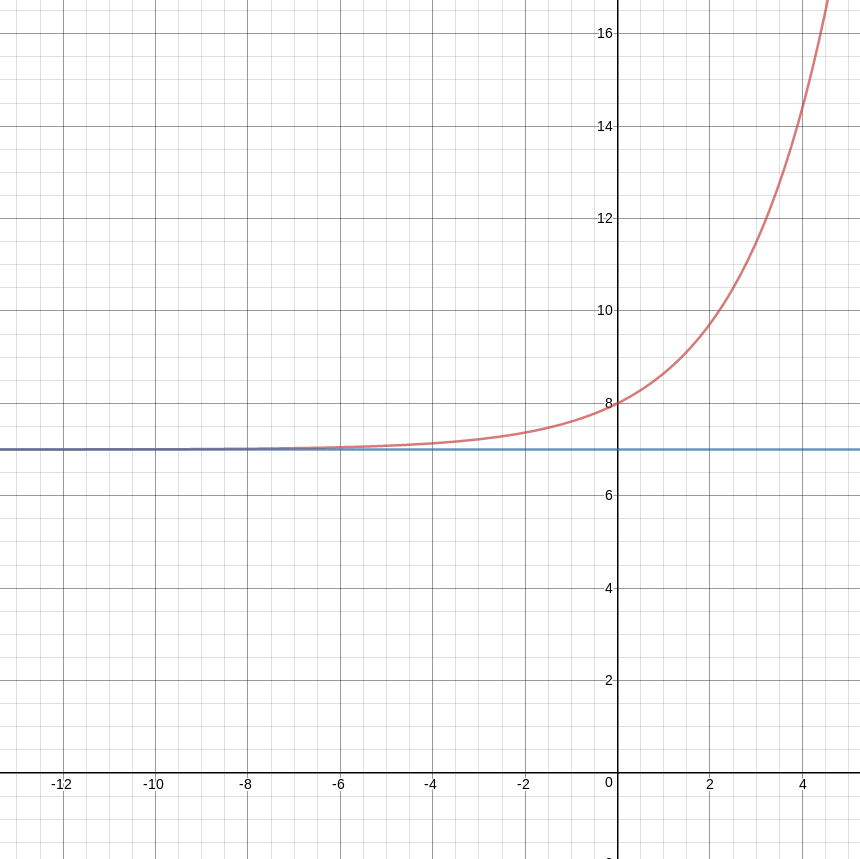
\includegraphics[scale=.25]{./asymp3.png}
\end{figure}
\end{frame}

\begin{frame}
  \frametitle{Finding Asymptotes II}
Example (this example additionally has two
  vertical asymptotes):
\begin{equation}
  \label{eq:ahyoimij}
  f(x)=\frac{\pi{}x^{2}+2x-1}{-7x^{2}+3x}\mbox{ has asymptotes }y=-\frac{e}{7},x=\frac{22}{7},x=0
\end{equation}
\begin{figure}[h]
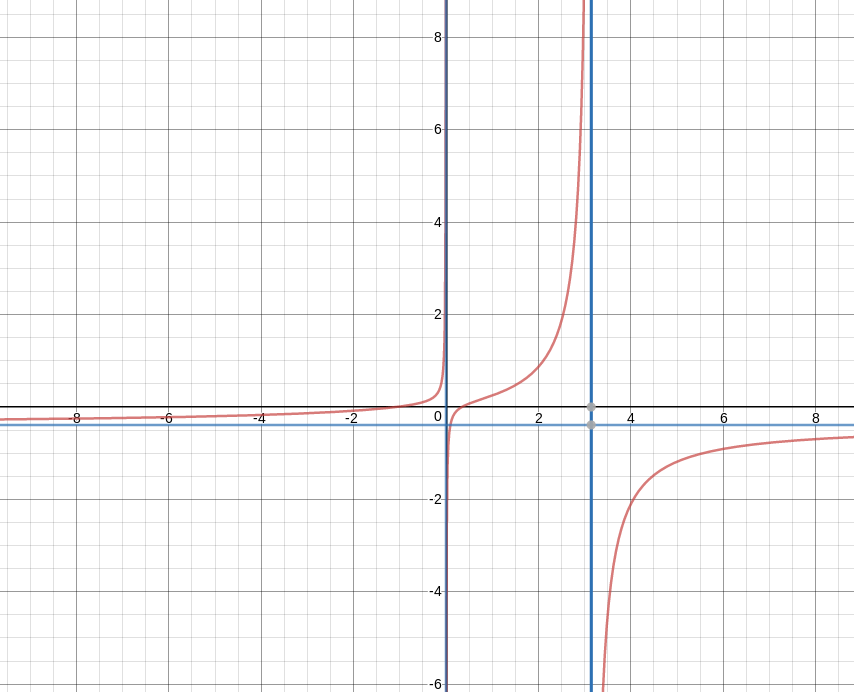
\includegraphics[scale=.25]{./asymp4.png}
\end{figure}
\end{frame}

\begin{frame}
  \frametitle{Finding Asymptotes III}
\begin{block}{Sloped Asymptote}
  A sloped asymptote is a linear function with a positive or a
  negative slope, $y=kx+d$ with $k\neq{}0$. There are sloped
  asymptotes for rational functions where the numerator polynomial's
  degree exceeds the denominator polynomial's degree by 1.
\end{block}
Find sloped asymptotes by checking
\begin{equation}
  \label{eq:uzuwooba}
  \lim_{x\rightarrow\infty}f'(x)\mbox{ and }\lim_{x\rightarrow{}-\infty}f'(x)
\end{equation}
If the limit is $k\neq{}0$, then that is also the slope of the
asymptote. Hyperbolas also sometimes have sloped asymptotes. 
\end{frame}

\begin{frame}
  \frametitle{Finding Asymptotes III}
Example:
\begin{equation}
  \label{eq:iboohoht}
  f(x)=\frac{3x^{2}-6x+2}{5x+4}\mbox{ has the asymptote }y=\frac{3}{5}x-\frac{5}{3}
\end{equation}
\begin{figure}[h]
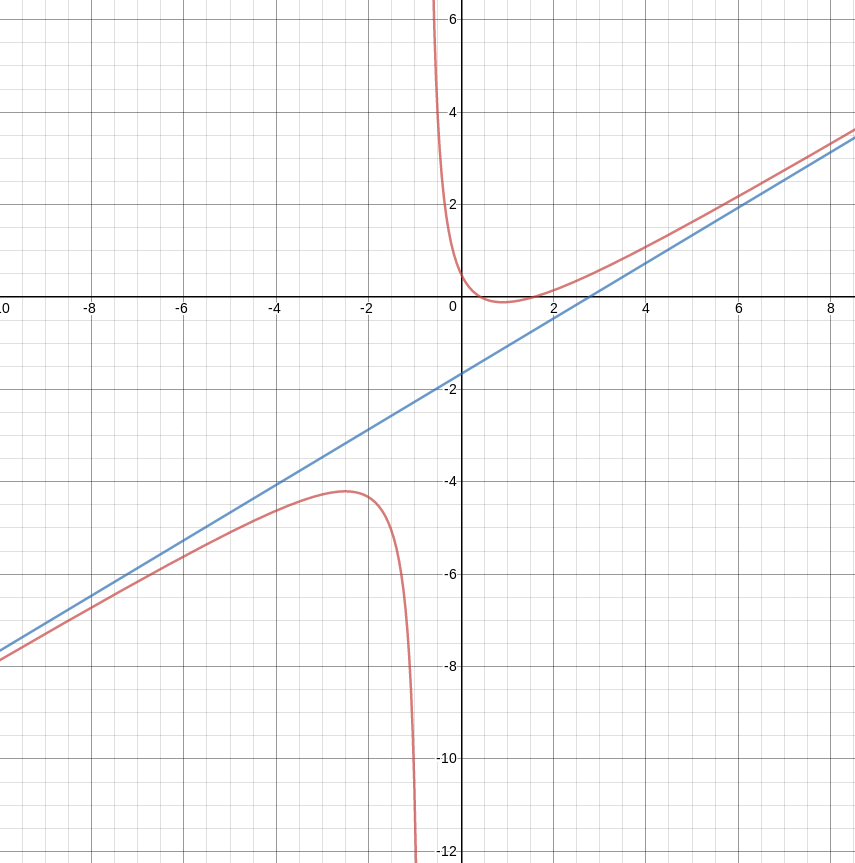
\includegraphics[scale=.25]{./asymp5.png}
\end{figure}
\end{frame}

% \begin{frame}
%   \frametitle{Finding Asymptotes III}
% Example:
% \begin{equation}
%   \label{eq:waduoqui}
%   f(\vartheta)=\sinh\vartheta
% \end{equation}
% \begin{figure}[h]
% 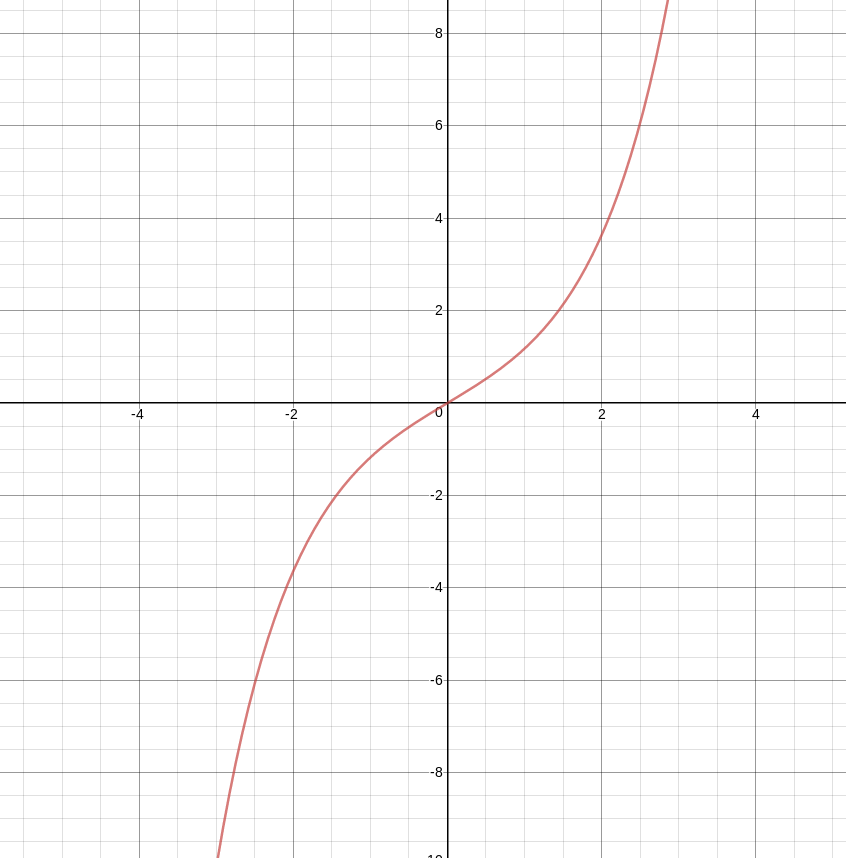
\includegraphics[scale=.25]{./asymp6.png}
% \end{figure}
% \end{frame}

\begin{frame}
  \frametitle{Analyzing Functions Exercises}
Analyze the following functions:
\begin{equation}
  \label{eq:ohkaedoy}
g_{1}(x)=-x^{2}+3x
\end{equation}
\begin{equation}
  \label{eq:teecakie}
g_{2}(x)=3x^{\frac{2}{3}}-2x
\end{equation}
\begin{equation}
  \label{eq:saepaego}
g_{3}(x)=\frac{2t^{2}}{t^{2}+3}
\end{equation}
\begin{equation}
  \label{eq:xohsaemu}
g_{4}(x)=x^{3}e^{x}
\end{equation}
\end{frame}

\begin{frame}
  \frametitle{Analyzing Functions Exercises Graph}
  \begin{figure}[h]
    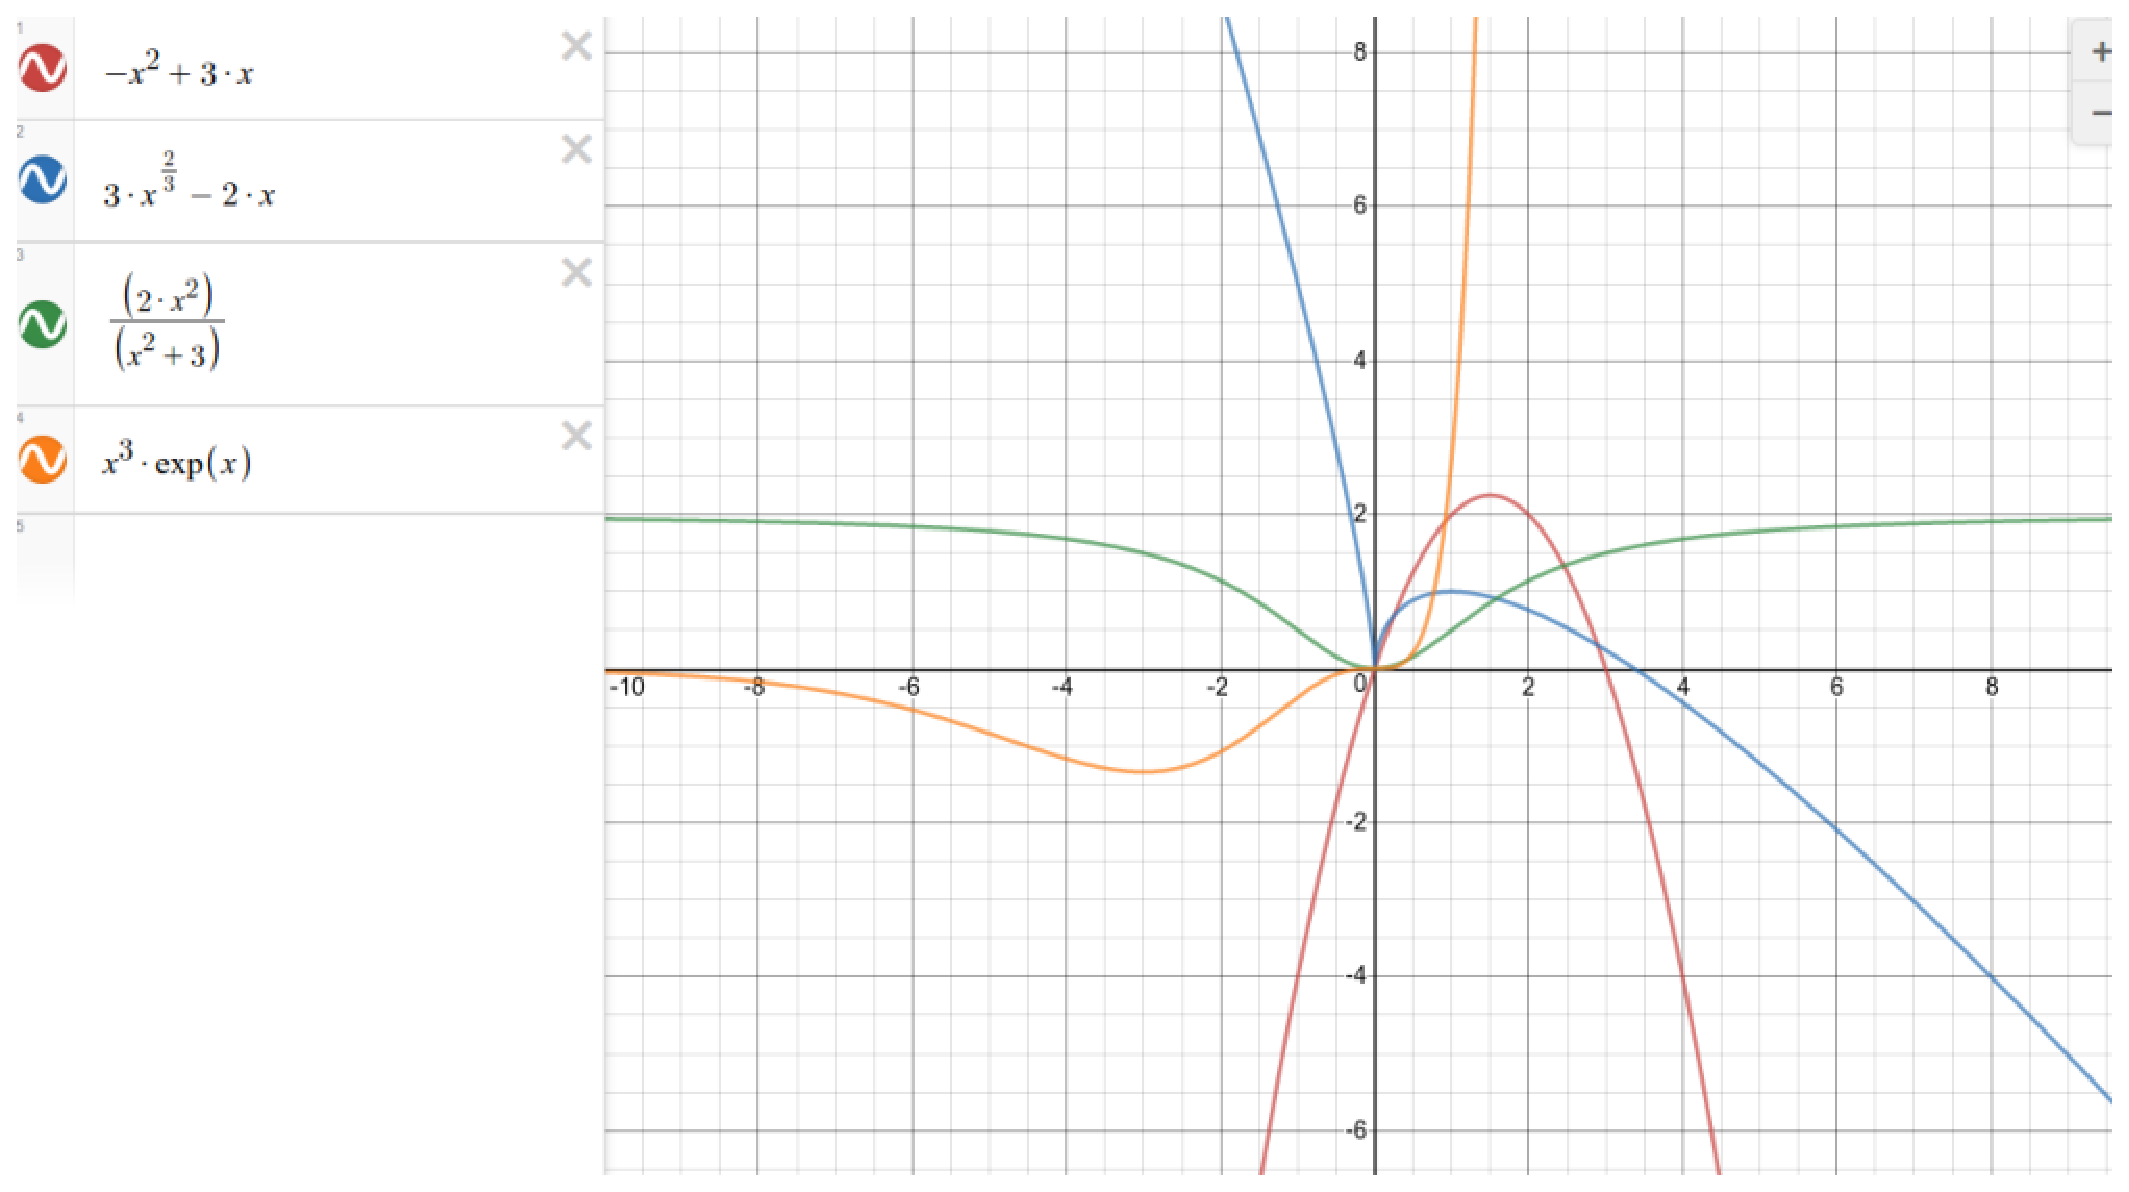
\includegraphics[scale=.4]{./ft-11-AnalyzingFunctions.eps}
  \end{figure}
\end{frame}

\begin{frame}
  \frametitle{End of Lesson}
Next Lesson: Analyzing Functions
\end{frame}

\end{document}

